\documentclass[
11pt, % The default document font size, options: 10pt, 11pt, 12pt
codirector, % Uncomment to add a codirector to the title page
]{charter} 




% El títulos de la memoria, se usa en la carátula y se puede usar el cualquier lugar del documento con el comando \ttitle
\titulo{\vspace{10px}Desarrollo de una nariz electrónica \vspace{10px} cuantificación de cianobacterias a través de inteligencia Artificial} 

% Nombre del posgrado, se usa en la carátula y se puede usar el cualquier lugar del documento con el comando \degreename
\posgrado{Carrera de Especialización en Intelegencia Artificial} 
%\posgrado{Carrera de Especialización en Internet de las Cosas} 
%\posgrado{Carrera de Especialización en Intelegencia Artificial}
%\posgrado{Maestría en Sistemas Embebidos} 
%\posgrado{Maestría en Internet de las cosas}

% Tu nombre, se puede usar el cualquier lugar del documento con el comando \authorname
\autor{Ing. Angela Siles} 

% El nombre del director y co-director, se puede usar el cualquier lugar del documento con el comando \supname y \cosupname y \pertesupname y \pertecosupname
\director{Nombre del Director}
\pertenenciaDirector{pertenencia} 
% FIXME:NO IMPLEMENTADO EL CODIRECTOR ni su pertenencia
\codirector{John Doe} % para que aparezca en la portada se debe descomentar la opción codirector en el documentclass
\pertenenciaCoDirector{FIUBA}

% Nombre del cliente, quien va a aprobar los resultados del proyecto, se puede usar con el comando \clientename y \empclientename
\cliente{Ing. Isaac Rodriguez}
\empresaCliente{Einsted S.A}

% Nombre y pertenencia de los jurados, se pueden usar el cualquier lugar del documento con el comando \jurunoname, \jurdosname y \jurtresname y \perteunoname, \pertedosname y \pertetresname.
\juradoUno{Nombre y Apellido (1)}
\pertenenciaJurUno{pertenencia (1)} 
\juradoDos{Nombre y Apellido (2)}
\pertenenciaJurDos{pertenencia (2)}
\juradoTres{Nombre y Apellido (3)}
\pertenenciaJurTres{pertenencia (3)}
 
\fechaINICIO{25 de abril de 2023}		%Fecha de inicio de la cursada de GdP \fechaInicioName
\fechaFINALPlan{13 de junio de 2023} 	%Fecha de final de cursada de GdP
\fechaFINALTrabajo{8 de febrero de 2024}	%Fecha de defensa pública del trabajo final


\begin{document}

\maketitle
\thispagestyle{empty}
\pagebreak


\thispagestyle{empty}
{\setlength{\parskip}{0pt}
\tableofcontents{}
}
\pagebreak


\section*{Registros de cambios}
\label{sec:registro}


\begin{table}[ht]
\label{tab:registro}
\centering
\begin{tabularx}{\linewidth}{@{}|c|X|c|@{}}
\hline
\rowcolor[HTML]{C0C0C0} 
Revisión & \multicolumn{1}{c|}{\cellcolor[HTML]{C0C0C0}Detalles de los cambios realizados} & Fecha      \\ \hline
0      & Creación del documento                                 &\fechaInicioName \\ \hline
%1      & Se completa hasta el punto 4 inclusive                 & dd/mm/aaaa \\ \hline
%2      & Se completa hasta el punto 7 inclusive
%		  Se puede agregar algo más \newline
%		  En distintas líneas \newline
%		  Así                                                    & dd/mm/aaaa \\ \hline
%3      & Se completa hasta el punto 11 inclusive                & dd/mm/aaaa \\ \hline
%4      & Se completa el plan	                                 & dd/mm/aaaa \\ \hline
\end{tabularx}
\end{table}

\pagebreak

%git--comment

\section*{Acta de constitución del proyecto}
\label{sec:acta}

\begin{flushright}
Buenos Aires, \fechaInicioName
\end{flushright}

\vspace{2cm}

Por medio de la presente se acuerda con el Ing. \authorname\hspace{1px} que su Trabajo Final de la \degreename\hspace{1px} se titulará ``Desarrollo de una nariz electrónica cuantificación de cianobacterias a través de inteligencia Artificial'', consistirá esencialmente en \textcolor{black}{la implementación de un prototipo de un sistema de detección de cianobacterias}, y tendrá un presupuesto preliminar estimado de \textcolor{black}{600} h de trabajo, con fecha de inicio \fechaInicioName\hspace{1px} y fecha de presentación pública \fechaFinalName.

Se adjunta a esta acta la planificación inicial.

\vfill

% Esta parte se construye sola con la información que hayan cargado en el preámbulo del documento y no debe modificarla
\begin{table}[ht]
\centering
\begin{tabular}{ccc}
\begin{tabular}[c]{@{}c@{}}Dr. Ing. Ariel Lutenberg \\ Director posgrado FIUBA\end{tabular} & \hspace{2cm} & \begin{tabular}[c]{@{}c@{}}\clientename \\ \empclientename \end{tabular} \vspace{2.5cm} \\ 
\multicolumn{3}{c}{\begin{tabular}[c]{@{}c@{}} \supname \\ Director del Trabajo Final\end{tabular}} \vspace{2.5cm} \\
%\begin{tabular}[c]{@{}c@{}}\jurunoname \\ Jurado del Trabajo Final\end{tabular}     &  & \begin{tabular}[c]{@{}c@{}}\jurdosname\\ Jurado del Trabajo Final\end{tabular}  \vspace{2.5cm}  \\
%\multicolumn{3}{c}{\begin{tabular}[c]{@{}c@{}} \jurtresname\\ Jurado del Trabajo Final\end{tabular}} \vspace{.5cm}                                                                     
\end{tabular}
\end{table}




\section{1. Descripción técnica-conceptual del proyecto a realizar}
\label{sec:descripcion}

El objetivo principal del proyecto es la detección temprana de cianobacterias en la República Argentina, debido a su potencial impacto negativo en la salud humana y en la economía del país. Estas bacterias pueden causar enfermedades en animales y seres humanos, así como la pérdida de cultivos y ganado, resultando en importantes pérdidas económicas. Actualmente, la falta de metodologías rápidas y precisas dificulta su control y prevención. Por lo tanto, se propone la implementación de dos sistemas de sensado complementarios para la detección en tiempo real de la presencia de cianobacterias.

La detección temprana de cianobacterias es crucial para prevenir su propagación y reducir su impacto en la salud humana y en la economía. La implementación de estos sistemas de sensado permitirá una detección rápida, precisa y confiable de cianobacterias en diferentes masas de agua, lo que permitirá a las autoridades tomar medidas preventivas a tiempo. Además, estos sistemas también ayudarán a identificar la especie de cianobacteria presente en la muestra de agua, lo que permitirá una respuesta más efectiva y específica ante su presencia.

El primer sistema se basa en la medición de los gases volátiles orgánicos emitidos por las capas concentradas de cianobacterias. Se emplearán sensores MOS (Metal Oxide Semiconductor) para detectar estos gases, y se utilizará una nariz electrónica equipada con un sistema de inteligencia artificial para procesar y analizar la información obtenida.

El segundo sistema consiste en el análisis visual de imágenes de controles positivos y negativos. Se realizará un análisis de las características visuales de las cianobacterias, utilizando un algoritmo de inteligencia artificial para identificar y diferenciarlas de otros organismos o materiales presentes en las muestras.

En el diagrama de bloques de la Figura 1, se observa que el sistema consta de dos bloques principales. El primer bloque, denominado "Análisis de gases", está compuesto por tres etapas:
\begin{itemize}
	\item Compresor: En esta etapa, el efluente se comprime para facilitar su análisis en las etapas posteriores.
	\item Sensor MOS: En esta etapa, se utilizan sensores MOS para detectar los gases volátiles orgánicos emitidos por las capas concentradas de cianobacterias.
	\item Nariz electrónica con sistema de inteligencia artificial: En esta etapa, se utiliza una nariz electrónica que procesa y analiza la información obtenida por los sensores MOS. El sistema de inteligencia artificial permite la identificación y cuantificación de los gases detectados, lo que permite una detección rápida y eficiente de la presencia de cianobacterias.
\end{itemize}
El segundo bloque del sistema, denominado "Análisis de imágenes", consta de dos etapas principales:

\begin{itemize}
\item Captura de imágenes: En esta etapa, se utilizan cámaras para capturar imágenes de controles positivos y negativos de cianobacterias.
\item Procesamiento de imágenes: En esta etapa, se procesan las imágenes capturadas utilizando un algoritmo de inteligencia artificial para identificar y diferenciar las cianobacterias de otros organismos o materiales presentes en las muestras.
\end{itemize}

Ambos bloques serán implementados y evaluados para determinar su efectividad en la detección de cianobacterias. Se espera que la combinación de estos sistemas permita una detección más rápida, precisa y confiable, contribuyendo así a prevenir los efectos negativos que las cianobacterias pueden tener en la salud humana y en la economía.

\begin{figure}[htpb]
\centering 
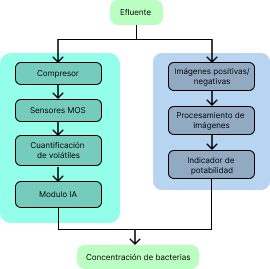
\includegraphics[width=.5\textwidth]{./Figuras/diagramaenbloque.png}
\caption{Diagrama en bloques del sistema}
\label{fig:diagBloques}
\end{figure}




\section{2. Identificación y análisis de los interesados}
\label{sec:interesados}

 
\begin{table}[ht]
%\caption{Identificación de los interesados}
%\label{tab:interesados}
\begin{tabularx}{\linewidth}{@{}|l|X|X|l|@{}}
\hline
\rowcolor[HTML]{C0C0C0} 
Rol           & Nombre y Apellido & Organización 	& Puesto 	\\ \hline
Auspiciante   & PhD. Nahuel Olaiz                  & \empclientename              	&CIO        	\\ \hline
Cliente       & \clientename      &\empclientename	& Desarrollador de hardware       	\\ \hline
Responsable   & \authorname       & FIUBA        	& Alumno 	\\ \hline
Orientador    & \supname	      & \pertesupname 	& Director Trabajo final \\ \hline
\end{tabularx}
\end{table}

 \begin{itemize}
	\item Auspiciante: PhD. Nahuel Olaiz, CIO \& CoFunder de EINSTED S.A, es quien aprueba todas las compras respectivas en cualquier proyecto.
	\item Cliente: Ing. Isaac Rodriguez, quien además es beneficiario de este proyecto para aplicar este sistema y se desempeña como desarrollador hardware de una sofisticada solución tecnológica.
	\item Responsable: Ing. Angela Siles, autora del proyecto de posgrado y empleada de EINSTED S.A bajo el cargo de Ingeniera Electrónica y Desarrolladora Front-end.
	\item Orientador: Nombre del director  
\end{itemize}

\section{3. Propósito del proyecto}
\label{sec:proposito}

	El propósito de este proyecto es desarrollar un sistema de monitoreo en línea para la detección y control de cianobacterias en cuerpos de agua. Se busca mejorar la calidad del agua y prevenir la propagación de estas bacterias nocivas para la salud y el ecosistema. Además, se implementarán tecnologías avanzadas para la recolección y análisis de datos en tiempo real.

\section{4. Alcance del proyecto}
\label{sec:alcance}

El presente proyecto a nivel hardware parte de las siguientes condiciones:

\begin{itemize}
	\item Incluirá todo lo necesario para el desarrollo del sistema, como microcontroladores, módulos de comunicación, soportes de carcasas impresión 3D, sensores y otros componentes específicos que deben ser reutilizados como requerimiento del cliente.
	\item Se realizará una revisión exhaustiva de los componentes existentes y se identificarán los que son necesarios para la implementación del sistema.
	\item Se realizará la adquisición de los componentes que sean necesarios para el correcto funcionamiento del sistema, tomando en cuenta los requisitos de calidad y disponibilidad.
\end{itemize}

En terminos de software la propuesta incluye:

\begin{itemize}
	\item El firmware permitirá que el hardware establecido sea operado por medio de un microcontrolador NodeMCU, y se realizará todo el sistema de control de sensores MOS.
	\item El software de usuario consiste en una aplicación de escritorio destinada para el cliente. Esta se comunicará con el firmware del sistema para dar información en tiempo real sobre la presencia de cianobacterias.

\end{itemize}


\section{5. Supuestos del proyecto}
\label{sec:supuestos}

Para el desarrollo del presente proyecto se supone que:

\begin{itemize}
\item Se contarán con los recursos financieros necesarios para la adquisición de los materiales y tecnología requeridos.
\item Se dispondrá del tiempo suficiente para llevar a cabo el desarrollo del proyecto según el cronograma establecido.
\item El equipo de trabajo asignado al proyecto contará con las habilidades y conocimientos necesarios para el desarrollo de las tareas.
\item La tecnología y los materiales a utilizar estarán disponibles en el mercado y serán accesibles para la adquisición en el momento requerido.
\item Las condiciones macroeconómicas y reglamentarias no afectarán significativamente el desarrollo del proyecto.
\end{itemize}

De no cumplirse los supuestos anteriores, se utilizarán datos similares, provenientes de otras fuentes.

\section{6. Requerimientos}
\label{sec:requerimientos}

\begin{consigna}{red}
Los requerimientos deben numerarse y de ser posible estar agruparlos por afinidad, por ejemplo:

\begin{enumerate}
	\item Requerimientos funcionales
		\begin{enumerate}
			\item El sistema debe...
			\item Tal componente debe...
			\item El usuario debe poder...
		\end{enumerate}
	\item Requerimientos de documentación
		\begin{enumerate}
			\item Requerimiento 1
			\item Requerimiento 2 (prioridad menor)
		\end{enumerate}
	\item Requerimiento de testing...
	\item Requerimientos de la interfaz...
	\item Requerimientos interoperabilidad...
	\item etc...
\end{enumerate}

Leyendo los requerimientos se debe poder interpretar cómo será el proyecto y su funcionalidad.

Indicar claramente cuál es la prioridad entre los distintos requerimientos y si hay requerimientos opcionales. 

No olvidarse de que los requerimientos incluyen a las regulaciones y normas vigentes!!!

Y al escribirlos seguir las siguientes reglas:
\begin{itemize}
	\item Ser breve y conciso (nadie lee cosas largas). 
	\item Ser específico: no dejar lugar a confusiones.
	\item Expresar los requerimientos en términos que sean cuantificables y medibles.
\end{itemize}

\end{consigna}

\section{7. Historias de usuarios (\textit{Product backlog})}
\label{sec:backlog}

\begin{consigna}{red}
Descripción: En esta sección se deben incluir las historias de usuarios y su ponderación (\textit{history points}). Recordar que las historias de usuarios son descripciones cortas y simples de una característica contada desde la perspectiva de la persona que desea la nueva capacidad, generalmente un usuario o cliente del sistema. La ponderación es un número entero que representa el tamaño de la historia comparada con otras historias de similar tipo.

El formato propuesto es: "como [rol] quiero [tal cosa] para [tal otra cosa]."

Se debe indicar explícitamente el criterio para calcular los \textit{story points} de cada historia
\end{consigna}

\section{8. Entregables principales del proyecto}
\label{sec:entregables}

\begin{consigna}{red}

Los entregables del proyecto son (ejemplo):

\begin{itemize}
	\item Manual de uso
	\item Diagrama de circuitos esquemáticos
	\item Código fuente del firmware
	\item Diagrama de instalación
	\item Informe final
	\item etc...
\end{itemize}

\end{consigna}

\section{9. Desglose del trabajo en tareas}
\label{sec:wbs}

\begin{consigna}{red}
El WBS debe tener relación directa o indirecta con los requerimientos.  Son todas las actividades que se harán en el proyecto para dar cumplimiento a los requerimientos. Se recomienda mostrar el WBS mediante una lista indexada:

\begin{enumerate}
\item Grupo de tareas 1
	\begin{enumerate}
	\item Tarea 1 (tantas h)
	\item Tarea 2 (tantas hs)
	\item Tarea 3 (tantas h)
	\end{enumerate}
\item Grupo de tareas 2
	\begin{enumerate}
	\item Tarea 1 (tantas h)
	\item Tarea 2 (tantas h)
	\item Tarea 3 (tantas h)
	\end{enumerate}
\item Grupo de tareas 3
	\begin{enumerate}
	\item Tarea 1 (tantas h)
	\item Tarea 2 (tantas h)
	\item Tarea 3 (tantas h)
	\item Tarea 4 (tantas h)
	\item Tarea 5 (tantas h)
	\end{enumerate}
\end{enumerate}

Cantidad total de horas: (tantas h)

Se recomienda que no haya ninguna tarea que lleve más de 40 h. 

\end{consigna}

\section{10. Diagrama de Activity On Node}
\label{sec:AoN}

\begin{consigna}{red}
Armar el AoN a partir del WBS definido en la etapa anterior. 

%La figura \ref{fig:AoN} fue elaborada con el paquete latex tikz y pueden consultar la siguiente referencia \textit{online}:

%\url{https://www.overleaf.com/learn/latex/LaTeX_Graphics_using_TikZ:_A_Tutorial_for_Beginners_(Part_3)\%E2\%80\%94Creating_Flowcharts}

\end{consigna}

\begin{figure}[htpb]
\centering 
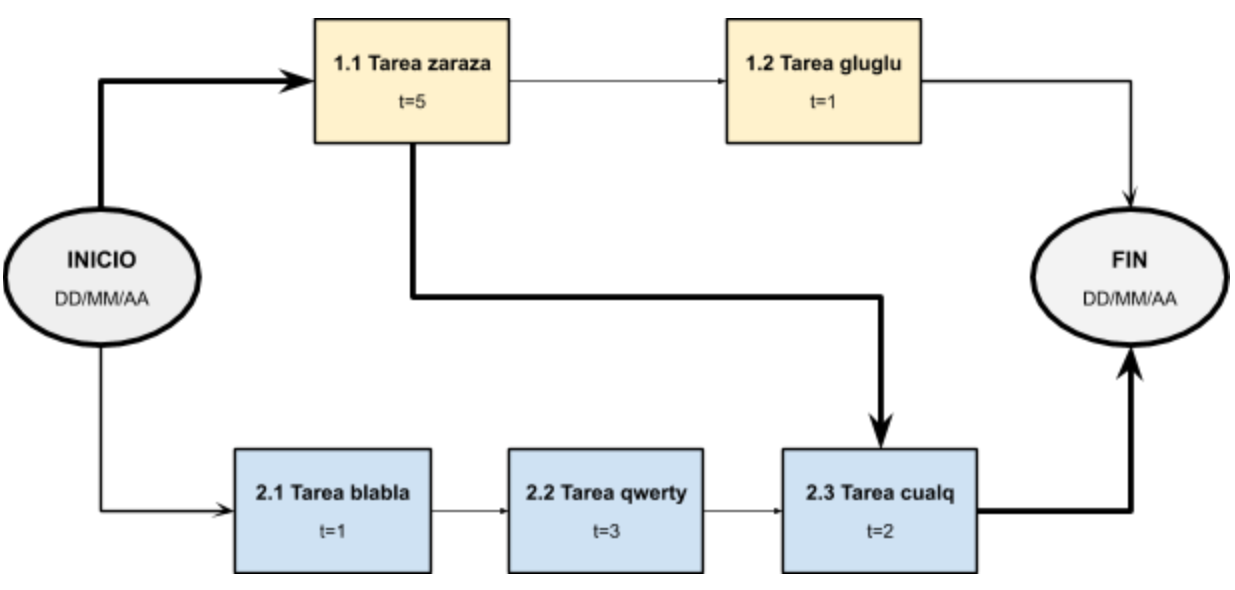
\includegraphics[width=.8\textwidth]{./Figuras/AoN.png}
\caption{Diagrama de \textit{Activity on Node}.}
\label{fig:AoN}
\end{figure}

Indicar claramente en qué unidades están expresados los tiempos.
De ser necesario indicar los caminos semicríticos y analizar sus tiempos mediante un cuadro.
Es recomendable usar colores y un cuadro indicativo describiendo qué representa cada color, como se muestra en el siguiente ejemplo:



\section{11. Diagrama de Gantt}
\label{sec:gantt}

\begin{consigna}{red}

Existen muchos programas y recursos \textit{online} para hacer diagramas de Gantt, entre los cuales destacamos:

\begin{itemize}
\item Planner
\item GanttProject
\item Trello + \textit{plugins}. En el siguiente link hay un tutorial oficial: \\ \url{https://blog.trello.com/es/diagrama-de-gantt-de-un-proyecto}
\item Creately, herramienta online colaborativa. \\\url{https://creately.com/diagram/example/ieb3p3ml/LaTeX}
\item Se puede hacer en latex con el paquete \textit{pgfgantt}\\ \url{http://ctan.dcc.uchile.cl/graphics/pgf/contrib/pgfgantt/pgfgantt.pdf}
\end{itemize}

Pegar acá una captura de pantalla del diagrama de Gantt, cuidando que la letra sea suficientemente grande como para ser legible. 
Si el diagrama queda demasiado ancho, se puede pegar primero la ``tabla'' del Gantt y luego pegar la parte del diagrama de barras del diagrama de Gantt.

Configurar el software para que en la parte de la tabla muestre los códigos del EDT (WBS).\\
Configurar el software para que al lado de cada barra muestre el nombre de cada tarea.\\
Revisar que la fecha de finalización coincida con lo indicado en el Acta Constitutiva.

En la figura \ref{fig:gantt}, se muestra un ejemplo de diagrama de Gantt realizado con el paquete de \textit{pgfgantt}. En la plantilla pueden ver el código que lo genera y usarlo de base para construir el propio.

\begin{figure}[htbp]
\begin{center}
\begin{ganttchart}{1}{12}
  \gantttitle{2020}{12} \\
  \gantttitlelist{1,...,12}{1} \\
  \ganttgroup{Group 1}{1}{7} \\
  \ganttbar{Task 1}{1}{2} \\
  \ganttlinkedbar{Task 2}{3}{7} \ganttnewline
  \ganttmilestone{Milestone o hito}{7} \ganttnewline
  \ganttbar{Final Task}{8}{12}
  \ganttlink{elem2}{elem3}
  \ganttlink{elem3}{elem4}
\end{ganttchart}
\end{center}
\caption{Diagrama de Gantt de ejemplo}
\label{fig:gantt}
\end{figure}


\begin{landscape}
\begin{figure}[htpb]
\centering 
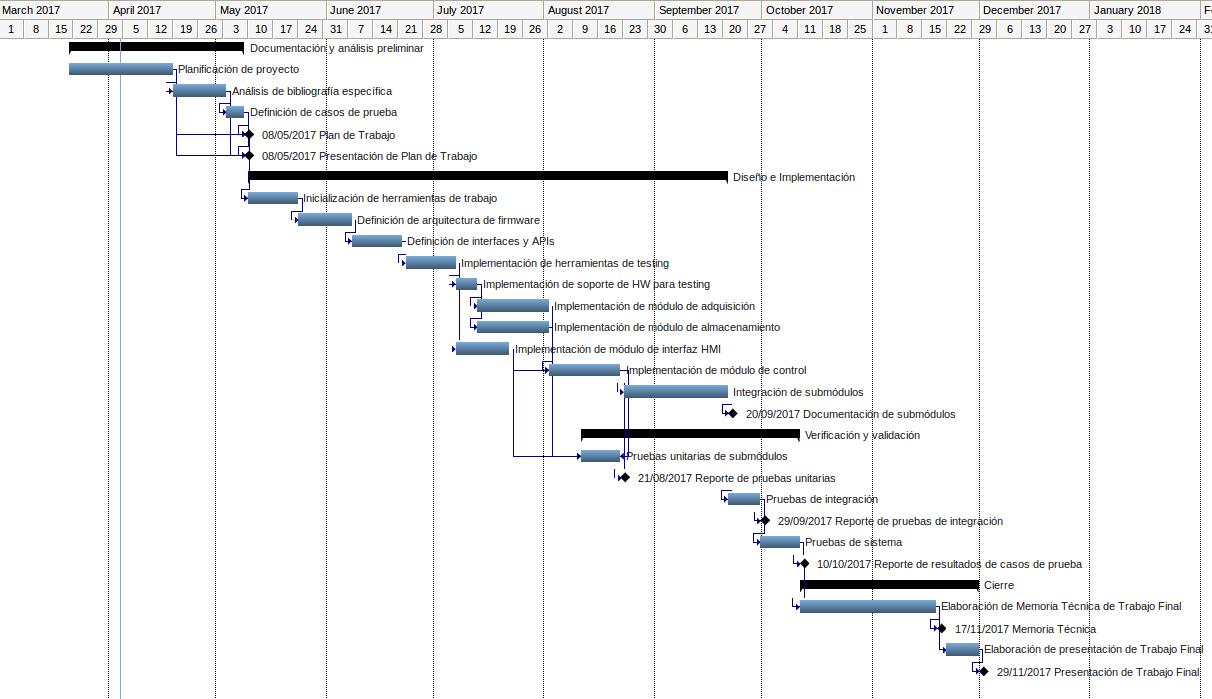
\includegraphics[height=.85\textheight]{./Figuras/Gantt-2.png}
\caption{Ejemplo de diagrama de Gantt rotado}
\label{fig:diagGantt}
\end{figure}

\end{landscape}

\end{consigna}


\section{12. Presupuesto detallado del proyecto}
\label{sec:presupuesto}

\begin{consigna}{red}
Si el proyecto es complejo entonces separarlo en partes:
\begin{itemize}
	\item Un total global, indicando el subtotal acumulado por cada una de las áreas.
	\item El desglose detallado del subtotal de cada una de las áreas.
\end{itemize}

IMPORTANTE: No olvidarse de considerar los COSTOS INDIRECTOS.

\end{consigna}

\begin{table}[htpb]
\centering
\begin{tabularx}{\linewidth}{@{}|X|c|r|r|@{}}
\hline
\rowcolor[HTML]{C0C0C0} 
\multicolumn{4}{|c|}{\cellcolor[HTML]{C0C0C0}COSTOS DIRECTOS} \\ \hline
\rowcolor[HTML]{C0C0C0} 
Descripción &
  \multicolumn{1}{c|}{\cellcolor[HTML]{C0C0C0}Cantidad} &
  \multicolumn{1}{c|}{\cellcolor[HTML]{C0C0C0}Valor unitario} &
  \multicolumn{1}{c|}{\cellcolor[HTML]{C0C0C0}Valor total} \\ \hline
 &
  \multicolumn{1}{c|}{} &
  \multicolumn{1}{c|}{} &
  \multicolumn{1}{c|}{} \\ \hline
 &
  \multicolumn{1}{c|}{} &
  \multicolumn{1}{c|}{} &
  \multicolumn{1}{c|}{} \\ \hline
\multicolumn{1}{|l|}{} &
   &
   &
   \\ \hline
\multicolumn{1}{|l|}{} &
   &
   &
   \\ \hline
\multicolumn{3}{|c|}{SUBTOTAL} &
  \multicolumn{1}{c|}{} \\ \hline
\rowcolor[HTML]{C0C0C0} 
\multicolumn{4}{|c|}{\cellcolor[HTML]{C0C0C0}COSTOS INDIRECTOS} \\ \hline
\rowcolor[HTML]{C0C0C0} 
Descripción &
  \multicolumn{1}{c|}{\cellcolor[HTML]{C0C0C0}Cantidad} &
  \multicolumn{1}{c|}{\cellcolor[HTML]{C0C0C0}Valor unitario} &
  \multicolumn{1}{c|}{\cellcolor[HTML]{C0C0C0}Valor total} \\ \hline
\multicolumn{1}{|l|}{} &
   &
   &
   \\ \hline
\multicolumn{1}{|l|}{} &
   &
   &
   \\ \hline
\multicolumn{1}{|l|}{} &
   &
   &
   \\ \hline
\multicolumn{3}{|c|}{SUBTOTAL} &
  \multicolumn{1}{c|}{} \\ \hline
\rowcolor[HTML]{C0C0C0}
\multicolumn{3}{|c|}{TOTAL} &
   \\ \hline
\end{tabularx}%
\end{table}


\section{13. Gestión de riesgos}
\label{sec:riesgos}

\begin{consigna}{red}
a) Identificación de los riesgos (al menos cinco) y estimación de sus consecuencias:
 
Riesgo 1: detallar el riesgo (riesgo es algo que si ocurre altera los planes previstos de forma negativa)
\begin{itemize}
	\item Severidad (S): mientras más severo, más alto es el número (usar números del 1 al 10).\\
	Justificar el motivo por el cual se asigna determinado número de severidad (S).
	\item Probabilidad de ocurrencia (O): mientras más probable, más alto es el número (usar del 1 al 10).\\
	Justificar el motivo por el cual se asigna determinado número de (O). 
\end{itemize}   

Riesgo 2:
\begin{itemize}
	\item Severidad (S): 
	\item Ocurrencia (O):
\end{itemize}

Riesgo 3:
\begin{itemize}
	\item Severidad (S): 
	\item Ocurrencia (O):
\end{itemize}


b) Tabla de gestión de riesgos:      (El RPN se calcula como RPN=SxO)

\begin{table}[htpb]
\centering
\begin{tabularx}{\linewidth}{@{}|X|c|c|c|c|c|c|@{}}
\hline
\rowcolor[HTML]{C0C0C0} 
Riesgo & S & O & RPN & S* & O* & RPN* \\ \hline
       &   &   &     &    &    &      \\ \hline
       &   &   &     &    &    &      \\ \hline
       &   &   &     &    &    &      \\ \hline
       &   &   &     &    &    &      \\ \hline
       &   &   &     &    &    &      \\ \hline
\end{tabularx}%
\end{table}

Criterio adoptado: 
Se tomarán medidas de mitigación en los riesgos cuyos números de RPN sean mayores a...

Nota: los valores marcados con (*) en la tabla corresponden luego de haber aplicado la mitigación.

c) Plan de mitigación de los riesgos que originalmente excedían el RPN máximo establecido:
 
Riesgo 1: plan de mitigación (si por el RPN fuera necesario elaborar un plan de mitigación).
  Nueva asignación de S y O, con su respectiva justificación:
  - Severidad (S): mientras más severo, más alto es el número (usar números del 1 al 10).
          Justificar el motivo por el cual se asigna determinado número de severidad (S).
  - Probabilidad de ocurrencia (O): mientras más probable, más alto es el número (usar del 1 al 10).
          Justificar el motivo por el cual se asigna determinado número de (O).

Riesgo 2: plan de mitigación (si por el RPN fuera necesario elaborar un plan de mitigación).
 
Riesgo 3: plan de mitigación (si por el RPN fuera necesario elaborar un plan de mitigación).

\end{consigna}


\section{14. Gestión de la calidad}
\label{sec:calidad}

\begin{consigna}{red}
Elija al menos diez requerientos que a su criterio sean los más importantes/críticos/que aportan más valor y para cada uno de ellos indique las acciones de verificación y validación que permitan asegurar su cumplimiento.

\begin{itemize} 
\item Req \#1: copiar acá el requerimiento.

\begin{itemize}
	\item Verificación para confirmar si se cumplió con lo requerido antes de mostrar el sistema al cliente. Detallar 
	\item Validación con el cliente para confirmar que está de acuerdo en que se cumplió con lo requerido. Detallar  
\end{itemize}

\end{itemize}

Tener en cuenta que en este contexto se pueden mencionar simulaciones, cálculos, revisión de hojas de datos, consulta con expertos, mediciones, etc.  Las acciones de verificación suelen considerar al entregable como ``caja blanca'', es decir se conoce en profundidad su funcionamiento interno.  En cambio, las acciones de validación suelen considerar al entregable como ``caja negra'', es decir, que no se conocen los detalles de su funcionamiento interno.

\end{consigna}

\section{15. Procesos de cierre}    
\label{sec:cierre}

\begin{consigna}{red}
Establecer las pautas de trabajo para realizar una reunión final de evaluación del proyecto, tal que contemple las siguientes actividades:

\begin{itemize}
	\item Pautas de trabajo que se seguirán para analizar si se respetó el Plan de Proyecto original:
	 - Indicar quién se ocupará de hacer esto y cuál será el procedimiento a aplicar. 
	\item Identificación de las técnicas y procedimientos útiles e inútiles que se emplearon, y los problemas que surgieron y cómo se solucionaron:
	 - Indicar quién se ocupará de hacer esto y cuál será el procedimiento para dejar registro.
	\item Indicar quién organizará el acto de agradecimiento a todos los interesados, y en especial al equipo de trabajo y colaboradores:
	  - Indicar esto y quién financiará los gastos correspondientes.
\end{itemize}

\end{consigna}


\end{document}
